%%---------------------------------------------------------------
%%---------------------------------------------------------------

\section{Firefox OS}

%%---------------------------------------------------------------

\begin{frame}
\frametitle{¿Qué es Firefox OS?}

\begin{itemize}
  \item Sistema operativo basado en Linux para \emph{smartphones} y tabletas
  \item Promovido por Mozilla (y otros \emph{partners} industriales, entre ellos Telefónica)
  \item Basado completamente en estándares abiertos: HTML5, CSS3 y JavaScript
  \item Incluye un modelo de privilegios y una API web abierta para comunicarse con el hardware del dispositivo
\end{itemize}

\end{frame}


%%---------------------------------------------------------------

\begin{frame}
\frametitle{La pila de Firefox OS}

\begin{center}
\begin{figure}[p]
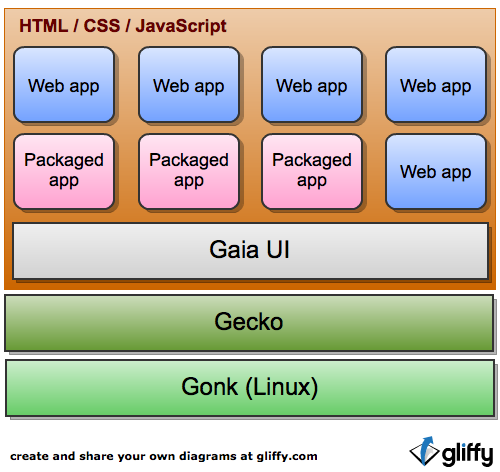
\includegraphics[width=0.65\textwidth]{figs/firefox-os-stack.png}
\end{figure}
\end{center}

\begin{flushright}
{\tiny
Source: http://kumar303.github.io/mozilla-apps-talk/images/firefox-os-stack.png
}
\end{flushright}

\end{frame}




%%---------------------------------------------------------------

\begin{frame}[fragile]
\frametitle{El manifiesto}

\begin{enumerate}
  \item El archivo \texttt{manifest.webapp} proporciona información importante sobre la aplicación
  \item Sólo el nombre y la descripción son obligatorios.
\end{enumerate}

\begin{footnotesize}
\begin{verbatim}
{
  "version": "0.1",
  "name": "Open Web App",
  "description": "Your new awesome Open Web App",
  "launch_path": "/app-template/index.html",
  "icons": {
    "16": "/app-template/app-icons/icon-16.png",
    "48": "/app-template/app-icons/icon-48.png",
    "128": "/app-template/app-icons/icon-128.png"
  },
  "developer": {
    "name": "Your Name",
    "url": "http://yourawesomeapp.com"
  },
  
\end{verbatim}
\end{footnotesize}
\end{frame}
  
%%---------------------------------------------------------------

\begin{frame}[fragile]
\frametitle{El manifiesto (y II)}  
  
\begin{footnotesize}
\begin{verbatim}
  "locales": {
    "es": {
      "description": "Su nueva aplicación impresionante Open Web",
      "developer": {
        "url": "http://yourawesomeapp.com"
      }
    },
    "it": {
      "description": "Il vostro nuovo fantastico Open Web App",
      "developer": {
        "url": "http://yourawesomeapp.com"
      }
    }
  },
  "default_locale": "en"
}
\end{verbatim}
\end{footnotesize}

\end{frame}

%%---------------------------------------------------------------

\begin{frame}
\frametitle{Tipos de Aplicaciones en Firefox OS}

\begin{enumerate}
  \item Empaquetadas: archivos .zip  conteniendo todos los archivos necesarios: HTML, CSS, JavaScript, imágenes, \texttt{manifest}, etc.
  \item Alojadas: en un servidor (con su URL). Requieren también un \texttt{manifest}.
\end{enumerate}

\end{frame}


%%---------------------------------------------------------------

\begin{frame}
\frametitle{WebAPIs}

\begin{center}
\begin{figure}[p]
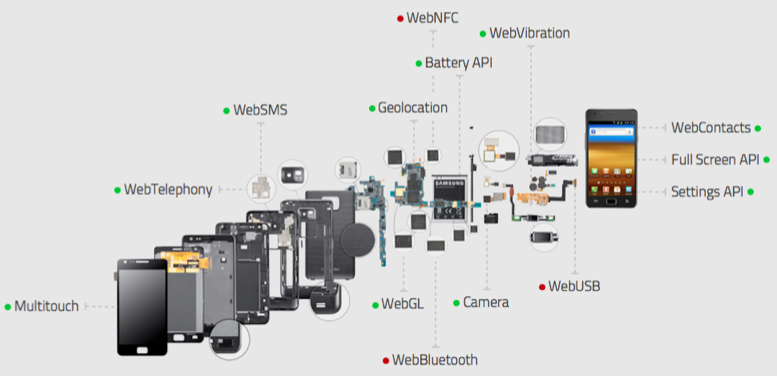
\includegraphics[width=0.99\textwidth]{figs/arewemobileyet.png}
\end{figure}
\end{center}

\begin{flushright}
{\tiny
Source: arewemobileyet.com
}
\end{flushright}

\end{frame}

%%---------------------------------------------------------------

\begin{frame}[fragile]
\frametitle{Web APIs}

\begin{itemize}
  \item APIs para interactuar con el \emph{hardware} de dispositivo
  \item Algunas APIs requieren permisos 
  \item Hay APIs previstas para el futuro
  \item Se puede ver un listado completo en \url{https://wiki.mozilla.org/WebAPI}
\end{itemize}

\begin{verbatim}
// If this device supports the vibrate API...
if('vibrate' in navigator) {
    // ... vibrate for a second
    navigator.vibrate(1000);
}
\end{verbatim}

\end{frame}


%%---------------------------------------------------------------

\begin{frame}
\frametitle{Permisos}

Hay tres tipos de APIs, según el tipo de permisos que hacen falta para ser ejecutadas, que
dan lugar a tres tipos de aplicaciones diferentes:

\begin{enumerate}
   \item Normales: APIs que no necesitan ningún tipo de permisos de acceso especiales.
   \item Privilegiadas: APIs disponibles para los desarrolladores para su uso en aplicaciones. Han de indicar los permisos de acceso en el manifiesto, y han de distribuirse a través de una fuente (\emph{app store}) de confianza.
   \item Certificadas: APIs que controlan funciones críticas en un dispositivo, como el marcador de llamadas y los servicios de mensajería. Estos por lo general no están disponibles para desarrolladores terceros.
\end{enumerate}

\end{frame}


%%---------------------------------------------------------------

\begin{frame}
\frametitle{Herramientas de desarrollo}

\begin{itemize}
  \item Firefox OS Simulator: integrable en Firefox \\
    \url{https://marketplace.firefox.com/developers/docs/firefox_os_simulator}
  \item App Manager: permite conectar Firefox a un dispositivo compatible con Firefox OS y enviar las aplicaciones para probarlas \\  
     \url{https://developer.mozilla.org/en-US/docs/Mozilla/Firefox_OS/Using_the_App_Manager}
  \item A partir de Firefox 33, \texttt{App Manaer} está siendo reemplazado por \texttt{WebIDE} \\
    \url{https://developer.mozilla.org/en-US/docs/Tools/WebIDE}
  \item Tests unitarios: QUnit (\url{http://qunitjs.com/})
\end{itemize}

\end{frame}


